% version 12
% Autor: Julian Salamanca
% Institución: Universidad Distrital Francisco José de Caldas
% Fecha: 09AGO2013
% Diego Alberto Parra Garzón 
\documentclass[jou]{apa6} %journal stilo APA con citacion clasica (apacite.pdf)
%\documentclass[doc]{apa6} % journal estilo latex
%\documentclass[man]{apa6}  % manuscrito APA

\usepackage[toc,page]{appendix}
\usepackage{balance}
\usepackage{multicol}
\usepackage{pdfpages}
\usepackage{afterpage}
\usepackage{float}
\usepackage{url}

\usepackage[spanish]{babel}
%\usepackage[latin1]{inputenc}% Tildes
\usepackage[utf8]{inputenc}
\usepackage{hyperref}
\urlstyle{same}

%====================================================================
%Para que no parta las palabras con guiones al final de linea
\usepackage[none]{hyphenat} 
\tolerance=6000
%====================================================================



%Stilo citaciones APA (debe ir despues de "hyperref ")
\usepackage{apacite} 

% para compilar eps con: pdflatex -shell-escape <archivo>.tex
\usepackage{epstopdf} 

\usepackage{amsmath, amsthm, amsfonts}
\usepackage{graphicx,wrapfig,lipsum}
\usepackage{anysize} 
\usepackage{fancyhdr}%
\pagestyle{fancy}
\marginsize{3cm}{3cm}{2,5cm}{2,5cm} 
%\fancypagestyle{empty}{

%  \setlength{\topmargin}{-0.5in}
%  \setlength{\headheight}{1.05in}
%  \setlength{\headsep}{0.5in}
%  \setlength{\headwidth}{\textwidth}
%  \setlength{\footskip}{2.0in}

 % \renewcommand{\headrulewidth}{0pt}

  % ========== EDITAR LOGO GRUPO =========================

%  \fancyhead[L]{
 %   \includegraphics[width=2.0cm, height=2.0cm]{LogoGI}
  %  \vspace{-1.0cm}
  %}
  % ========== FIN NO EDITAR LOGO GRUPO =================
  

  % ========== NO EDITAR LOGO UD =========================

%  \fancyhead[R]{
 %   \includegraphics[width=5.5cm, height=1.2cm]{img/logo_UD_EXT}
 % }
  % ========== FIN NO EDITAR ===========================
  

%}


\title{Prototipo GPS con software y hardware de libre acceso para transmisión de datos de geo-localización hacia las gafas smarth glass BT-300 de EPSON.}

\shorttitle{ARTICULO PROTOTIPO GPS SENA}

%==================== AUTOR (ES) ========================
\author{Lic. en Física Diego Alberto Parra Garzón \\ \href{mailto:{dparra@opensai.org}}{dparra@opensai.org}}
\date{\today}
\affiliation{OPENSAI, SENA}
\leftheader{Diego Parra}
%==================== FIN AUTOR (ES) ====================

%==================== RESUMEN ========================
\abstract{
\begin{center}
\textbf{Abstrac}
\end{center}


The present writing done a description detailed and understandable the mounting of two prototype GPS for the transmission of geo-location data to the glasses smarth glass BT-300 EPSON; this due that sunglasses GPS sensor does not show the geo-location data as EPSON does not have good coverage satellite in Colombia due to the latitude where it is located, this confirmed the sr. Rafael Godinho Aranjues, Regional Business Manager EPSON Latin America (54) 11-5167-0404 rafael\_aranjues@epson.com.ar; the number one prototype has GPS, antenna 28 dB, thermometer, led processes, power supply of 5 V and Wi-Fi; the second prototype has Bluetooth, GPS with 28 dB antenna communications, thermometer, 16 x 4 LCD screen, processes, 5V and 9V power leds.


\emph{\textbf{Keywords:} } IoT, FreeSotfware, OpenSource, Science, Technology, GPS, Bluetooth, WIFI, Smarth Glass, EPSON.

\begin{center}
\textbf{Resumen}
\end{center}

El presente escrito realiza una descripción detalla y entendible del montaje de dos prototipos GPS para la transmisión de datos de geo-localización hacia las gafas smarth glass BT-300 de EPSON; esto debido a que el sensor GPS de las gafas no muestra los datos de geo-localización pues EPSON no tiene buena cobertura satelital en Colombia debido a la latitud en la que se encuentra, esto lo confirma el señor Rafael Godinho Aranjues, Regional Business Manager EPSON Latin America (+54) 11-5167-0404  rafael\_aranjues@epson.com.ar; el prototipo número uno cuenta con GPS, antena de 28 dB, termómetro, leds indicadores de procesos, alimentación de 5 V y conexión WIFI; el segundo prototipo cuenta con comunicación Bluetooth, GPS con antena de 28 dB, termómetro, pantalla LCD de 16x4,  leds indicadores de procesos, alimentación de 5 V y 9V.

\emph{\textbf{Palabras Claves:} } IoT, FreeSotfware, OpenSource, Ciencia, Tecnología, GPS, Bluetoth, WIFI, Smarth Glass, EPSON.

}

%==================== FIN RESUMEN ========================

\begin{document}

%================  NO EDITAR =================
\renewcommand{\tablename}{Tabla} %"Cuadro" por "Tabla"
\renewcommand{\refname}{Referencias} %"Cuadro" por "Tabla"
\def\st@rtbibsection{\mspart{Referencias}}% ``References'' por ``Referencias'
\renewcommand{\rheadname}{Encabezado de página}% Running head (encabezado de pagina)
\renewcommand{\acksname}{Nota de Autor}% 
\renewcommand{\keywordname}{Palabras clave}% 
\renewcommand{\listtablename}{Índice de tablas}% 
\renewcommand{\BOthers}[1]{et al.\hbox{}}
\renewcommand{\appendixname}{Ap} %"Cuadro" por "Tabla"
\renewcommand{\appendixname}{Anexo}
\renewcommand{\appendixname}{Anexos}
\renewcommand{\appendixtocname}{Anexos}
\renewcommand{\appendixpagename}{Anexos}
\maketitle


%============== TABLA DE CONTENIDO ===============

\tableofcontents
\listoffigures
%\listoftables

%=================INTRODUCCION ============
\section{Introducción}
La realidad aumentada, es una tecnología emergente que ha sido introducida desde el ámbito militar  y científico hacia la vida diaria de cada persona; con ayuda de los dispositivos móviles se esta haciendo cada vez más popular esta tecnología, y, no solo en aplicaciones militares,  \cite{fombona2012realidad} sino también en los hogares, escuelas, universidades, múseos, centros de interés turístico, reservas forestales y  en cada sector de la sociedad; este gran avance acompañado de la curiosidad del ser humano y de grandes inventos como relojes, televisores, electrodomésticos y en general en la mayor parte de artefactos “inteligentes”; \cite{telefonica2011realidad} es por esto que la realidad aumentada es una nueva lente para ver el mundo e interactuar con el universo virtual a través de los sentidos y la  capacidad del ser humano para dejarse impresionar. 

En particular se observo que el proyecto de investigación aplicada y desarrollo tecnológico realizado por Opensai en asocio con el Centro de Gestión de Mercados, Logística y TI del SENA para el desarrollo de una solución especializada de seguimiento, control y administración para el sector logístico en bodegas de almacenaje; en sus especificaciones técnicas aparecen las gafas de Realidad Aumentada BT-300 de EPSON las cuales satisfacen la mayor parte de los requerimientos del proyecto, solo que en el desarrollo de la aplicación para las \texttt{smarth glass BT-300}, los datos de geo-posicionamiento que se solicitaban al dispositivo no eran recibidos por este instrumento tecnológico y al contactar con la empresa EPSON, ellos especificaron que la cobertura satelital de GPS para latitudes como la de Colombia, no llega de manera ideal; debido a estas razones el equipo Opensai decide desarrollar dos sistemas de transmisión de datos de posicionamiento geo-referenciado, los cuales se utilizan para transmitir dichos valores a las gafas y obtener el funcionamiento adecuado de la aplicación para solución de logística en bodegas de almacenaje.  

\section{\texttt{Prototipo WIFI}}

Como se observa en las figuras \ref{fig:Proto1-1} y \ref{fig:Proto12}, el prototipo WIFI fue realizado con un microcontrolador ATMEGA-328, el cual es el encargado de controlar la toma de datos del módulo \texttt{GPS-NEO 6m} como la adquisición de la lectura de sensación térmica de un termómetro LM-35 y enviar los datos vía serial al módulo WIFI ESP-8266, este microcontrolador ATMEGA-328 también realiza la función de controlar dos LED's, los cuales permiten identificar los procesos que lleva a cabo el microcontrolador; el módulo WIFI ESP-8266 envía los valores de posicionamiento y temperatura a una base de datos de tipo MYSQL como lo es PHPMYADMIN.

\begin{figure}[htb]
  \centering
\setlength\fboxsep{0pt}
\setlength\fboxrule{0.5pt}
\fbox{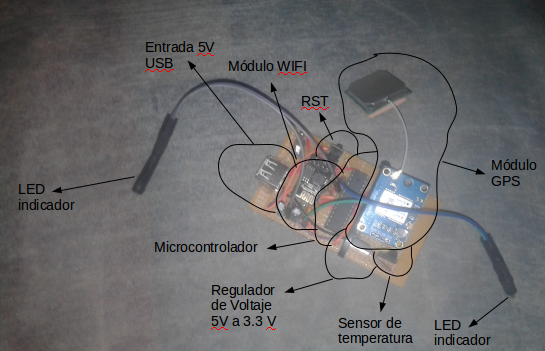
\includegraphics[width=7cm, height=5.0cm, angle=0]{PROTO1_1.png}}
  \caption{\footnotesize Prototipo GPS con salida de datos vía WIFI a una base de datos SQL. Fuente el autor 2017.}
  \label{fig:Proto1-1}  
\end{figure}

En la figura \ref{fig:Proto1-2} se aprecia el esquema eléctrico del circuito para el prototipo GPS, este cumple con los requisitos propuestos en primera instancia, como envío de los valores de latitud, longitud y temperatura a través de WIFI, que serán utilizados por la aplicación de las \texttt{smarth glass BT-300}, para realizar el mapeo del lugar y de esta manera orientar al usuario de la aplicación.

\begin{figure}[htb]
  \centering
\setlength\fboxsep{0pt}
\setlength\fboxrule{0.5pt}
\fbox{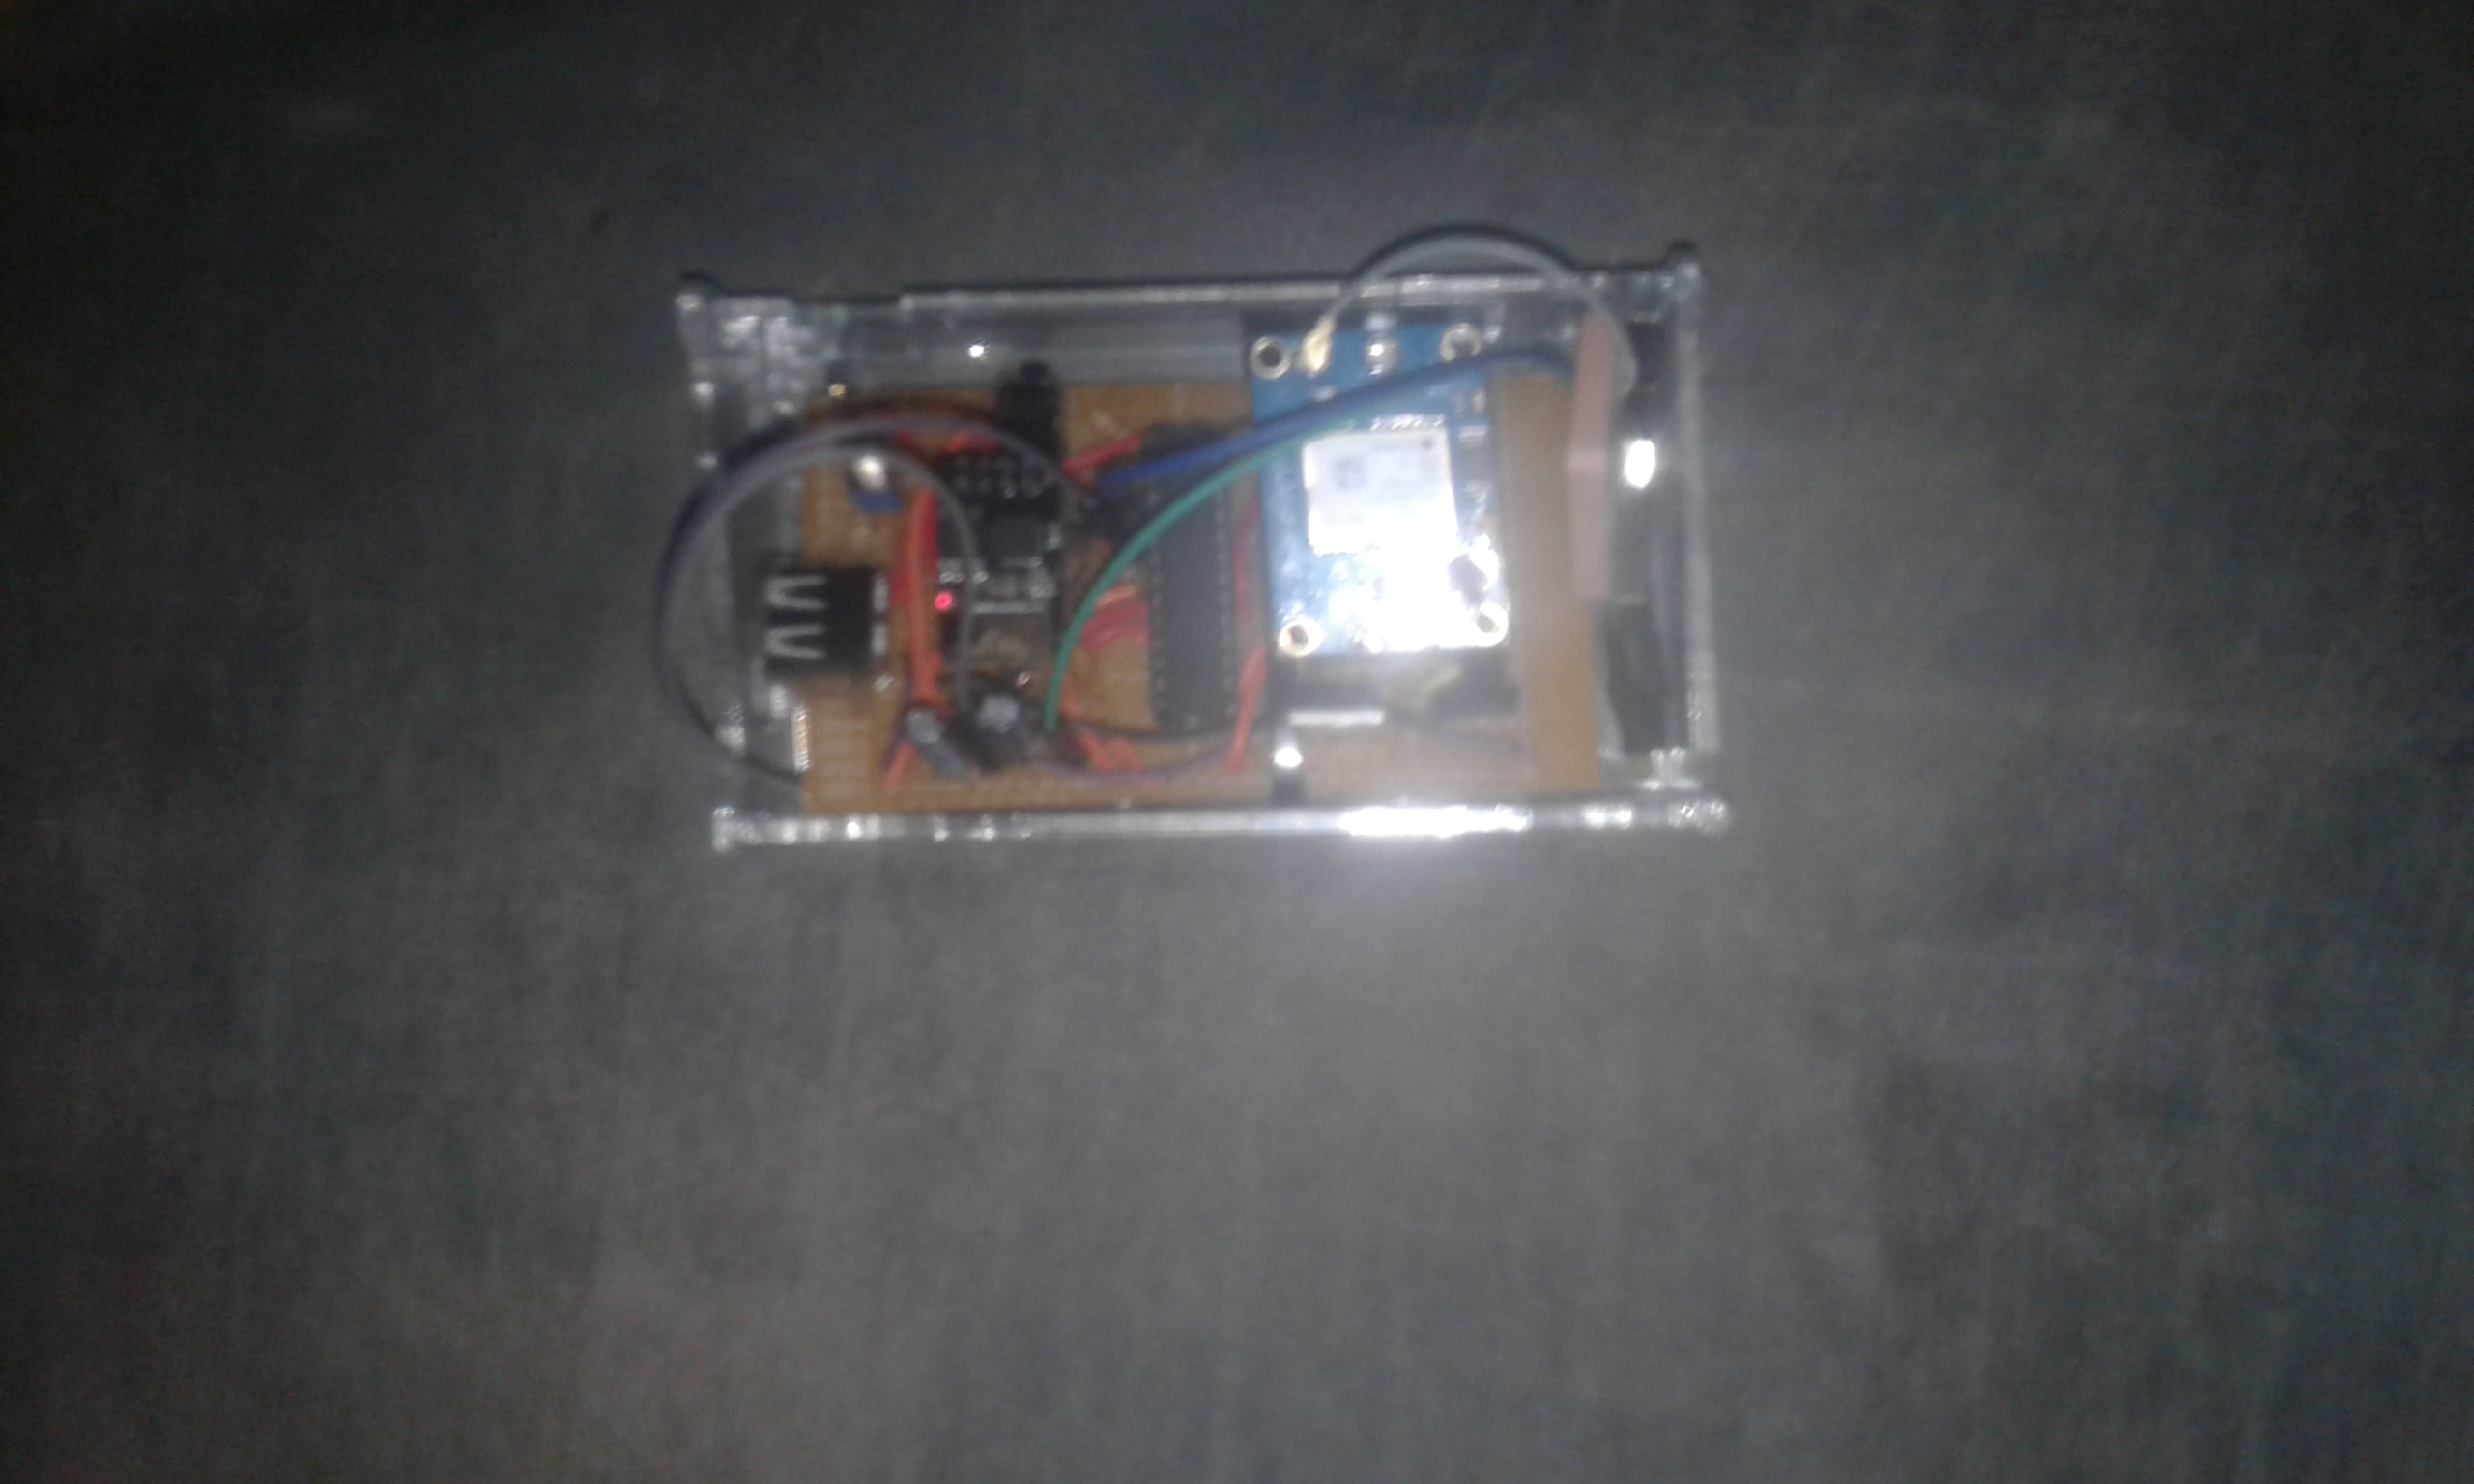
\includegraphics[width=7cm, height=5.0cm, angle=0]{Img/proto1_1.jpg}}
  \caption{\footnotesize Prototipo GPS WIFI en estuche de plástico para un arduino mega 2560. Fuente el autor 2017.}
  \label{fig:Proto12}  
\end{figure}

\begin{figure}[htb]
  \centering
\setlength\fboxsep{0pt}
\setlength\fboxrule{0.5pt}
\fbox{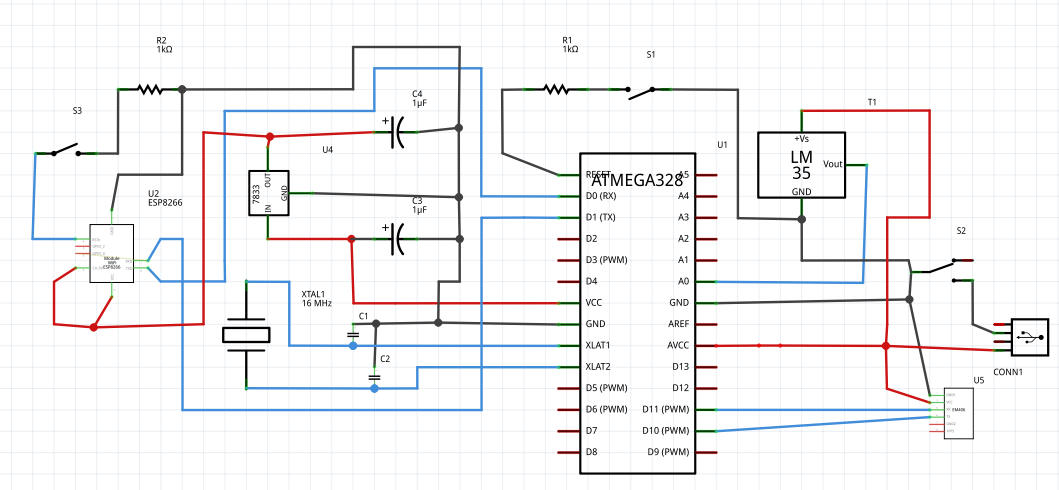
\includegraphics[width=7cm, height=5.0cm, angle=0]{Es_co.png}}
  \caption{\footnotesize Esquema eléctrico del prototipo GPS. Fuente el autor 2017.}
  \label{fig:Proto1-2}  
\end{figure}

%\subsection{'Esquema eléctrico'}


\bibliographystyle{apacite}
\bibliography{referencias}
\end{document}





